\section{WR Transparent Clocks}
\label{sec:wr_tc}
PTP Transparent Clock (TC) modifies PTP messages as they pass through them
adding the residence time to an accumulative Correction Field (CF) in the PTP 
messages. Thus, the delay introduced  by the network is measured and can be 
subtracted in the slave clock, which improves distribution accuracy.

In ~\ref{sec:wr} the WRPTP and WR synchronization steps have been described for
master, slave and boundary clocks. This chapter presents how a standard TC becomes a WR TC.

\begin{figure*}[!t]
\centering
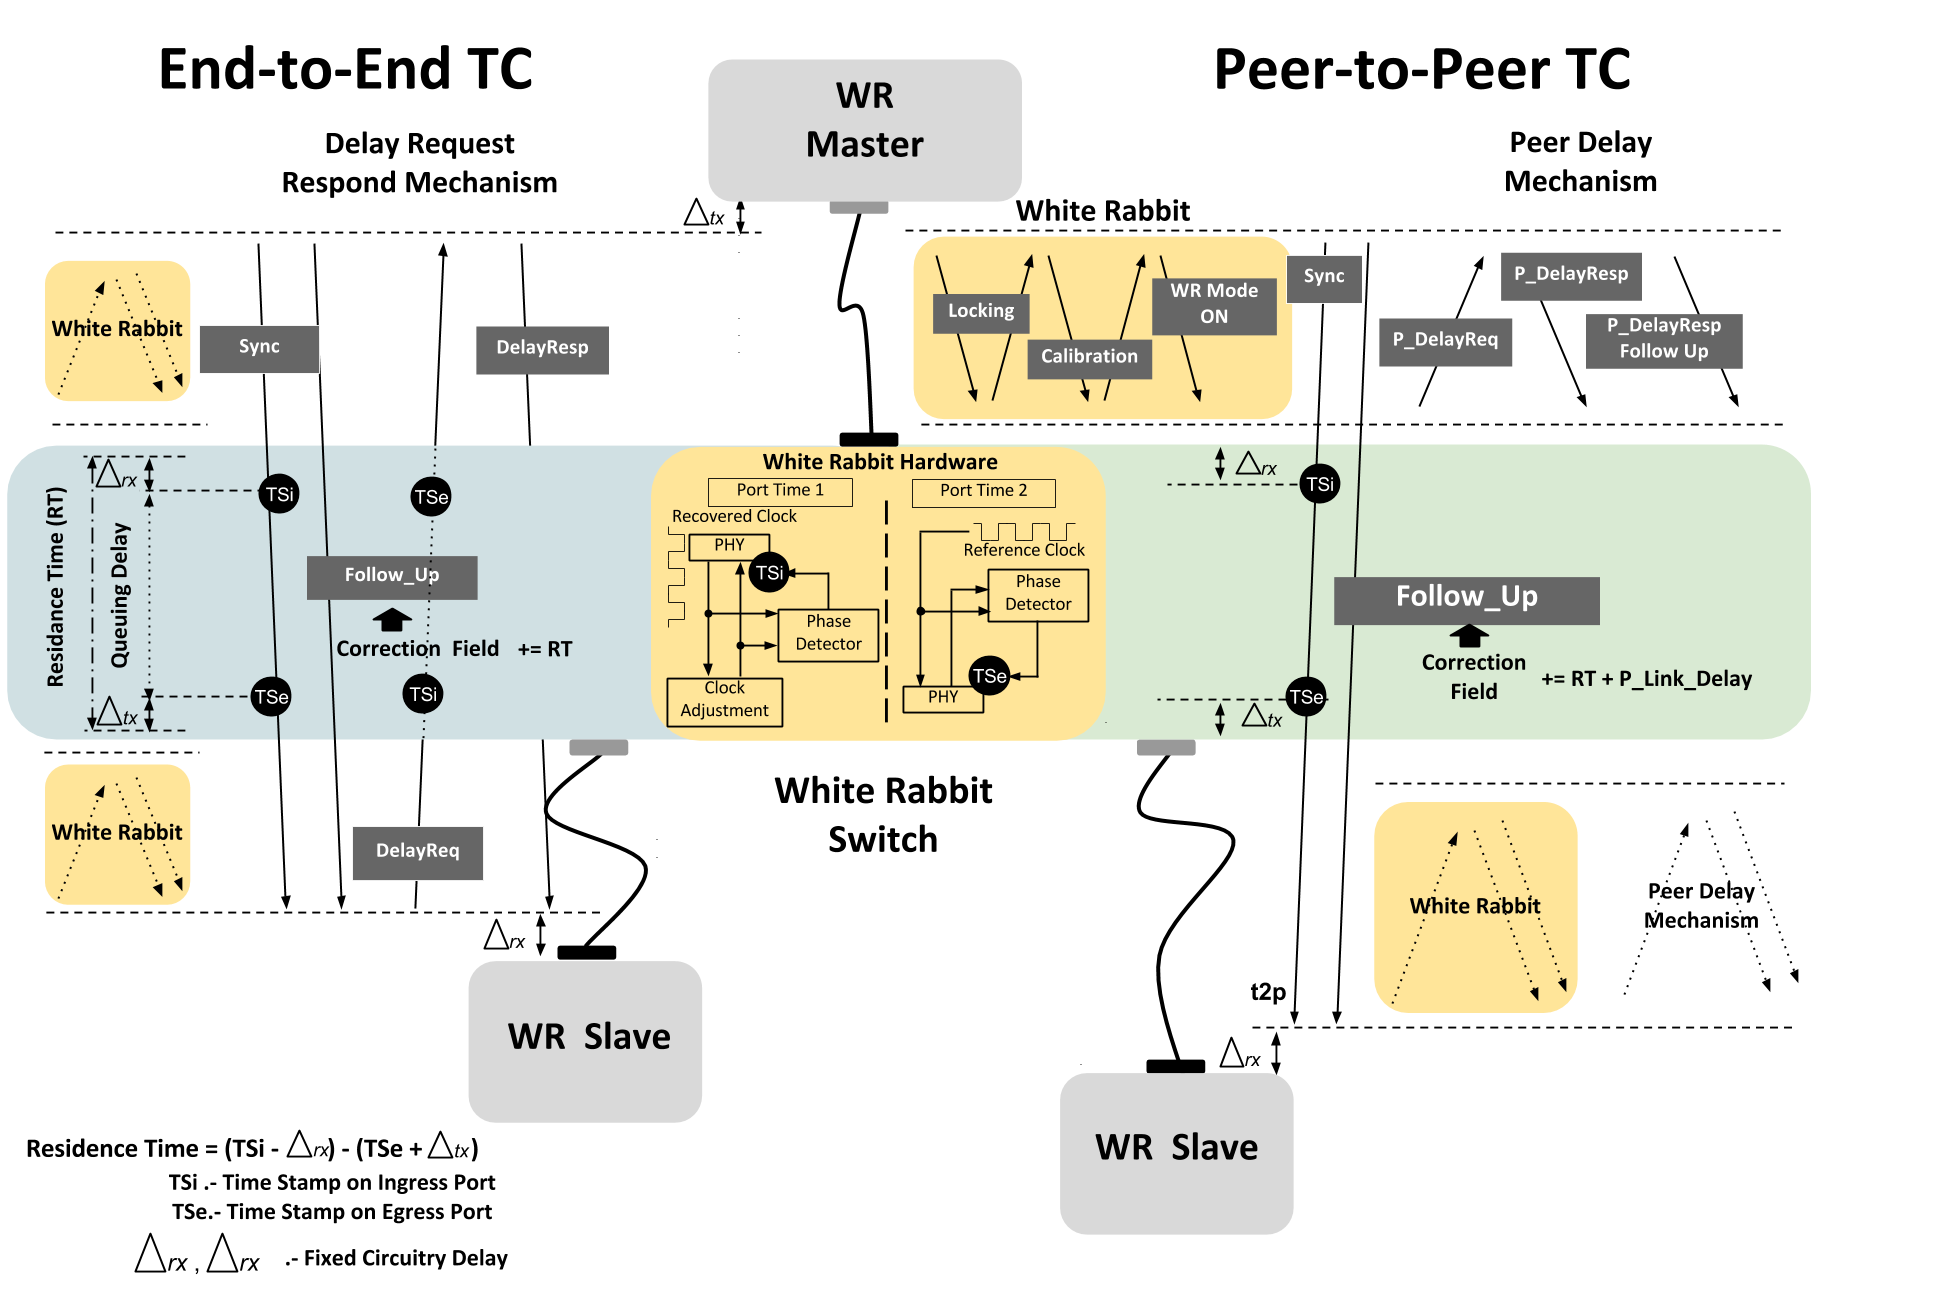
\includegraphics[scale=0.27]{fig/wr_schema_hw_bw.png}
\caption{WR End two End and Peer to Peer Transparent Clocks}
\label{fig:wr_tc}
\end{figure*}

%\subsection{End-to-End WR Transparent Clock}
%
%As the standard End-to-End (E2E) clocks, the WR E2E TC doesn't belong to the
%master-slave hierarchy and does not synchronized to the WR Master. 
%Therefore, a WR E2E accomplishes only the synthonization and the calibration.
%Thus the WR Mode is on without the $phase_{mm}$ or $phase_{s}$ measurement
%between the master and the slave, but between the slave and the adjacent WR
%Switch. 
%
%The \figurename~\ref{fig:wr_tc} shows the PTP exchange of messages from master to slave,
%going through the switch transparently and how the residence time is also calculated taking into 
%account the fixed delays $\Delta$. Thanks to the synthonization and fixed delay measurements done during 
%the WRPTP there is not error in the measurement of the residence time. A two-step WR E2E TC calculates, using
%(\ref{eq:delayms}), the $offset_{ms}$:
%
%\begin{equation}
%    \label{eq:residence_time}
%     CF += (TS_{ingess\_port} - \Delta_{rx}) -
%     (TS_{egress\_port} + \Delta_{tx})
%\end{equation}
%
%\begin{equation}
%    \label{eq:wre2e}
%     offset_{ms} = t_{1} - t_{2} - delay_{ms} - CF
%\end{equation}
%
\subsection*{Peer-to-Peer WR Transparent Clock}

As the standard Peer-to-Peer (P2P) clocks, the WR P2P TC measures residence time
of Sync messages, and the link delay in both directions. The
\figurename~\ref{fig:wr_time_stamp} and \figurename~\ref{fig:wr_tc}
show the PTP exchange of messages from master to slave going through the switch 
transparently and how the residence time is also calculated taking into  account the fixed delays $\Delta$. 


The link delay between master and slave is calculated according to~\eqref{eq:round_trip_2}:

\begin{equation}
  \label{eq:delayss_1}
    delay_{ss} = \Delta + \sigma _{ms} + \sigma _{sm}
\end{equation}

using the fiber asymmetry relation~\eqref{eq:disp}:

\begin{equation}
  \label{eq:delayss_2}
    delay_{ss} = \Delta + (1 + \alpha) \sigma _{sm} + \sigma _{sm}
\end{equation}

adding the fixed delays due to transmission circuitry:

\begin{equation}
    \label{eq:delaysm}
     delay_{sm} = \frac{delay_{ss} - \Delta}{2+ \alpha} + \Delta_{txs} +
     \Delta_{rxm} 
\end{equation}

Since the link delay is done between adjacent clocks using the peer delay mechanism, 
the full WR synchronization process can be issued between the two ports. 
The measurement of the residence time, like in the BC should suffer no error
since the ports are syntonized to its master clock, but also the measurement of the
link delays, are as precise as the WR project claims ~\cite{biblio:ispcs_m} for the
Boundary Clocks. The link delay is calculated like in \eqref{eq:delayms}, 
but using $t_{3}$, $t_{4p}$, $t_{5}$ and $t_{6p}$ instead. The $offset_{ms}$ is calculated:

\begin{equation}
    \label{eq:residence_time}
     residence\_time= (TS_{ingess\_port} - \Delta_{rx}) -
     (TS_{egress\_port} + \Delta_{tx})
\end{equation}


\begin{equation}
    \label{eq:wrp2p}
     CF += residance\_time + delay\_link
\end{equation}


\begin{equation}
    \label{eq:wrp2p_1}
     offset_{ms}= t_{1} - t_{2} - CF - delay\_link \footnote{This link delay
     corresponds to the last link to the slave}
\end{equation}

%\FloatBarrier
